\chapter{Literature Review}
\label{ch:1}

}

\hypertarget{conceptual-clarifications}{%
\section{\texorpdfstring{\textbf{1.1 Conceptual Clarifications}}{1.1 Conceptual Clarifications}}\label{conceptual-clarifications}}

\hypertarget{concept-of-urbanization}{%
\section{\texorpdfstring{\textbf{1.1.1 Concept of Urbanization}}{1.1.1 Concept of Urbanization}}\label{concept-of-urbanization}}

Urbanization is defined as the increasing concentration of people, infrastructure, and economic activities in towns and cities, resulting in the physical and demographic expansion of urban areas. Historically, it evolved alongside the industrialization in the past 18th and 19th centuries, as technological innovations, improved transportation, and factory-based economies drew populations from rural settlements into emerging metropolitan centers (Murayama and Estoque 2020) https://recentscientific.com/urbanization-concepts-dimensions-and-factors. But in our contemporary era, urbanization have shifted from being an industrial phenomenon to a global socio-economic process shaped by globalization, service economies, and technological transformation. This shift is especially concentrated (pronounced) in the most developing nations of the world, where urban growth is charaterized by unprecedented rates of human population increase and ofcourse it is often without corresponding improvements in infrastructure, environmental management, or governance (Bai et al. 2017; Waheeb 2023). Looking at the context of Africa and Asia, rapid urbanization is largely driven by natural population increase, rural-urban migration, expanding economic opportunities, informal settlements, and the physical extension of built-up land into peri-urban and agricultural zones(Gutu Sakketa 2023). Further more, the causes are majorly; the infrastructural development, political centralization, transportation corridors, and land speculation, all of which reinforce the conversion of natural landscapes into urban land uses (Longo et al. 2023; Li et al. 2016). The combination of these factors made urbanization (rapid urban growth) a powerful force to recogned with which is really shaping ecological patterns, resource availability, and environmental quality particularly in low- and middle-income regions where urban planning systems struggle to keep pace with population and spatial expansion.
\hypertarget{urbanization-in-the-tropical-context}{%
\section{\texorpdfstring{\textbf{1.1.2 Urbanization in the Tropical Context}}{1.1.2 Urbanization in the Tropical Context}}\label{urbanization-in-the-tropical-context}}

Urbanization in tropical regions is shaped by unique environmental, socio-economic, and climatic conditions that distinguish tropical cities from those in temperate zones. The major charaterictics of the tropical cities are; high population densities, rapid spatial expansion, extensive informal settlements, insufficient infrastructure, and strong dependence on natural resources and ecosystem services (Smith et al. 2020; He et al. 2021). The climate condition of these cities are marked by high temperature, intense rainfall, and also a year-round biological productivity heighten sensitivity to land-use change, making vegetation cover, soil properties, and hydrological systems particularly vulnerable to urban disturbances. The evidence from the humid tropical regions, is that the problem excalate to deforestation, altering of microclimates, reducing vegetation greenness, increasing of surface runoff, and degrading soil fertility (Yin et al. 2024), which in turn leads to significant ecological consequences such as biodiversity loss, reduced carbon storage, and weakened ecosystem (Yin et al. 2024; Ramil Abbasov 2025).
Across Africa, and particularly in West Africa, urban growth has been exceptionally on the high and is driven by natural population increase, rural-urban migration, administrative centralization, and expanding economic activities in transportation and trade (Kankam et al. 2024).According to previous studies (Kisvarga et al. 2023; Ogwu 2019), West African mega cities such as Lagos, Accra, Bamako, and the emerging secondary ones such as Makurdi and Otukpo clearly exhibit similar patterns of fragmented expansion, infrastructural deficits, and strong interactions between human activities and ecological processes.
\hypertarget{land-use-and-land-cover-lulc}{%
\section{\texorpdfstring{\textbf{1.1.3 Land Use and Land Cover (LULC)}}{1.1.3 Land Use and Land Cover (LULC)}}\label{land-use-and-land-cover-lulc}}

Land use refers to the human purposes or activities applied to the land such as agriculture, settlements, industry, transportation, and conservation reflecting socio-economic decisions and management practices imposed on the (Nedd, et al. 2021) and land cover describes the physical and biophysical features present on the Earth's surface, including vegetation, water bodies, bare soil, built-up areas, and wetlands, regardless of how humans utilize (Gaur and Singh 2023). While, the two are conceptually distinct, but are closely linked (land use influences land cover through activities like deforestation, cultivation, and urban development, and changes in land cover can shape future land-use decisions by determining resource availability, ecological suitability, and environmental (Da Silva et al. 2020)). According to Yaghoobi et al. 2022, it is vital to understand the linkges between human-induced land-use activities and the leading drivers of land-cover change globally, especially in rapidly urbanizing regions where natural landscapes are continuously converted into built-up surfaces (Yaghoobi et al. 2022).
Also, from past studies (Lou et al. 2025; Derdouri et al. 2021), accurate LULC mapping/classification can aid environmental managegers and researchers to quantify and evaluate the patterns of vegetation loss, habitat fragmentation, soil degradation, hydrological disruption, and urban expansion key processes that shape ecological responses at multiple spatial scales. To manage tropical and developing nations cities, where urban expansion is at the height and fast and often uncontrolled, LULC assessments are crucial for monitoring environmental impacts, planning green infrastructure, and implementing conservation strategies. Remote sensing and GIS in the other hand have become indispensable tools for proper and adequately LULC analysis, offering consistent, repeatable, and large-scale observations that support the evaluation of long-term ecological (Mohajane et al. 2018; Aryal et al. 2023). For studies like the present research, LULC dynamics provide the foundational spatial context for examining how urbanization gradients influence plant diversity, soil conditions, and vegetation productivity.
\hypertarget{urbanization-gradient}{%
\section{\texorpdfstring{\textbf{1.1.4 Urbanization Gradient}}{1.1.4 Urbanization Gradient}}\label{urbanization-gradient}}

The urbanization gradient referring to as a spatial continuum ranging from rural areas with low population density and minimal built infrastructure, through peri-urban areas which are characterized by a mixed land uses and rapid transformation, to highly developed urban centers dominated by impervious surfaces and intensive human activities (Seress et al. 2014). This particular urban gradient framework is becoming more commonly used in ecological research (Alue et al. 2022; Wu 2014; Ullah et al. 2025), because it captures the progressive influence of urban development on environmental phenomena, therefore allowing a systematic comparisons of biodiversity, ecosystem functions, and habitat quality across varying levels of human engaments (Barbieri et al. 2023).
\hypertarget{plant-diversity}{%
\section{\texorpdfstring{\textbf{1.1.5 Plant Diversity}}{1.1.5 Plant Diversity}}\label{plant-diversity}}

Plant diversity comprises several complementary dimensions which are: 1) species richness, 2) the sheer count of different plant species, 3) species evenness-referring to how equally individuals are distributed among those species; and broader metrics such as alpha diversity (diversity within a site), beta diversity (turnover or change in species composition between sites), and gamma diversity (total diversity across a landscape) (Vasilevich 2009; Zhang et al. 2023). These dimensions offers differently ecological insights and paths. For example, the α-diversity helps understand local community complexity, while the β-diversity reveals how plant composition shifts across environmental or land-use classes (Qi et al. 2024). High plant diversity plays a crucial role in ecosystem functioning and resilience. Major empirical studies (Toscano et al. 2025; Mogîldea and Biță-Nicolae 2024), have demonstrated that the greater species richness enhances carbon storage, boosts productivity, and improves multiple ecosystem services by promoting complementary resource management, stabilizing community structure, and increasing resistance to environmental stressor/disturbances. Kovacs et al. 2025 in their study of urban ecology, diverse plant communities support services such as air purification, microclimate regulation, pollinator habitats, and soil stabilization, making plant diversity a key component of sustainable and resilient city.
\hypertarget{ecosystem-functioning}{%
\section{\texorpdfstring{\textbf{1.1.6 Ecosystem Functioning}}{1.1.6 Ecosystem Functioning}}\label{ecosystem-functioning}}

Ecosystem functioning refers to the sum of ecological processes that regulate how ecosystems operate, including primary productivity, nutrient cycling, energy flow, soil formation, and vegetation (Mollashahi and Szymura 2022). These processes determine the capacity of ecosystems to sustain life and maintain stability, and even if they are strongly influenced by parameters such as soil organic matter, microbial activity, vegetation cover, and hydrological balance (Breuste et al. 2017). In terrestrial landscapes, indicators such as net primary productivity (NPP), soil nutrient availability, infiltration capacity, and biomass accumulation are commonly used to assess ecosystem functioning, especially in environments undergoing rapid land-use changes (Včeláková et al. 2023). A substantial collection of evidence has proven beyond doubt that biodiversity particularly of the plant species richness and functional diversity enhances ecosystem functioning by promoting complementary resource use, stabilizing productivity, and improving nutrient retention and soil (Onandia et al. 2019; Marques and Mandrak 2024). The biodiversity ecosystem functioning (BEF) relationship is majorly critical in most urbanized landscapes of tropical regions of the world, where habitat fragmentation and vegetation loss can impair carbon sequestration, nutrient cycling, and soil all at once (Gu et al. 2024)), making plant diversity a key driver of ecological integrity across rural-urban gradients.
\hypertarget{vegetation-indices-ndvi-evi}{%
\section{\texorpdfstring{\textbf{1.1.7 Vegetation Indices (NDVI, EVI)}}{1.1.7 Vegetation Indices (NDVI, EVI)}}\label{vegetation-indices-ndvi-evi}}

Vegetation indices are quantitative measures derived from satellite spectral reflectance, particularly the differential reflection of red and near-infrared (NIR) wavelengths by vegetation available all in Landsat and Sentinel imageries, which allow researchers and environmental managers to assess plant vigoriously and photosynthetic activity (Reddy and Prasad 2018). NDVI, basically operates on the principle that any healthy plants absorb red light for photosynthesis and strongly reflecting NIR radiation, producing values that correlate highly with biomass, productivity, and canopy (Benhizia et al. 2024)). EVI on ther other hand, builds on the limitations of NDVI by incorporating blue band reflectance and correction factors to minimize atmospheric interference and canopy background noise, making it more highly and reliable in humid or densely vegetated tropical (Gaikwad et al. 2025).Both, have become essential tools for evaluating plant ecosystem health, detecting vegetation stress, monitoring urbanization impacts, and quantifying changes in ecological functioning across landscapes especially in rapidly transforming tropical cities where field data alone are insufficient(Priya et al. 2023; Hassani et al. 2023). Their integration within a same GIS and remote sensing framework enhances the capacity to track reliable and efficient spatio-temporal vegetation patterns, providing robust indicators of ecological degradation, fragmentation, and resilience along urbanization gradients for accurately and acceptable results suitable for policy recommendations (Kamble et al. 2010).
\hypertarget{soil-ecosystem-indicators}{%
\section{\texorpdfstring{\textbf{1.1.8 Soil Ecosystem Indicators}}{1.1.8 Soil Ecosystem Indicators}}\label{soil-ecosystem-indicators}}

Soil ecosystem properties particularly (soil organic carbon (SOC), nitrogen (N), bulk density, pH, and electrical conductivity (EC)) are considered the fundamental measures of soil health and ecological functioning of any soil (Mattoo et al. 2025). SOC serves as a reservoir for a long-term carbon storage and the regulation of soil structure, water retention and nutrient availability, where nitrogen is critical and central to nutrient cycling and plant (Mattoo et al. 2025). Bulk density reflects soil compaction: higher bulk density, often found in urbanized areas, reduces porosity and limits root growth and microbial (Frene et al. 2024; Zhu et al. 2024). Soil pH influences microbial community composition and enzymatic processes, and it proven that urban soils frequently exhibit altered pH due to construction materials and pollution, which in turn affects nutrient (Almendro-Candel et al. 2018). Electrical conductivity provides a measure of soil salinity or ionic strength, influencing nutrient uptake by plants and soil organisms, particularly in degraded or engineered urban (Mu et al. 2024). Together, these indicators are critical because they link physical and chemical soil conditions to ecosystem processes such as carbon sequestration, nutrient cycling, and plant productivity, making them indispensable for assessing how urbanization degrades or transforms below-ground ecological (Macci et al. 2025)).
\hypertarget{urban-ecology}{%
\section{\texorpdfstring{\textbf{1.1.9 Urban Ecology}}{1.1.9 Urban Ecology}}\label{urban-ecology}}

City or urban ecology examines how cities as a novel of ecosystems that host human activities and profoundly shape the ecological structure and processes takes place. It is majorly characterized among other indicators by a mosaic of built infrastructure, green patches, remnant fragments, and highly modified environments, which create complex landscapes with unique microclimates and resource distributions all together (Byrne 2024). Fragmentation in real sense and according to (Tanner et al. 2014; Douglas 2017) is a pervasive outcome of urbanization where natural habitats are broken into smaller, isolated patches by roads, buildings, and other infrastructure, species movement, genetic flow, and ecological connectivity decline, contributing to biodiversity loss and functional homogenization. Anthropogenic pressures in the context of ecosystems go beyond fragmentation they include the following: pollution (air, light, noise), invasive species, and altered disturbance regimes, all of which reshuffle community composition toward generalist and disturbance-tolerant species (Wu 2014; McPhearson et al. 2016)2016). In tropical cities, where urban greening opportunities exist but planning is often weak, we can see these pressures combine to cause significant changes in ecological dynamics, making urban ecology a critical framework for understanding how human-dominated landscapes affect plant diversity, ecosystem functioning, and long-term environmental resilience.
\hypertarget{review-of-related-concepts-and-approaches}{%
\section{\texorpdfstring{\textbf{1.2 Review of Related Concepts and Approaches}}{1.2 Review of Related Concepts and Approaches}}\label{review-of-related-concepts-and-approaches}}

\hypertarget{land-use-land-cover-change-detection}{%
\section{\texorpdfstring{\textbf{1.2.1 Land Use / Land Cover Change Detection}}{1.2.1 Land Use / Land Cover Change Detection}}\label{land-use-land-cover-change-detection}}

LULC change detection is a cornerstone approach in ecological and urban research, involving the use of satellite imagery and remote sensing tools to effectively monitor and evaluate how far human activities and natural processes reshape the landscape over time and place. By leveraging multi-temporal satellite data (Landsat, Sentinel), researchers can map changes in built-up areas, vegetation, water, agriculture and other classes of LULC across decades, offering a retrospective view of urban expansion and ecological (Viana et al. 2019; Dadi et al. 2016). Two most widely used change detection techniques/approaches are post-classification comparison, where independently classified images from different dates are compared to produce ``from-to'' change maps, and supervised classification, in which training data (from ground truth or high-resolution imagery) guide pixel labeling into discrete land-use classes (Chughtai et al. 2021; Selvaraj and Nagarajan 2022). The post-classification methods often includes constructing transition matrices, which solely quantify how much area in size and percentage has converted from one class (forest) to another (built-up), allowing for clear interpretation of patterns such as urban sprawl or habitat loss (Mas et al. 2017). At a global scene, such methodology have demonstrated effieciently how growing urban cities expand in extent, rising impervious surfaces and leading to consequential loss of vegetated and cropland; locally, studies in Nigeria have employed supervised classification to document dramatic built-up growth at the expense of vegetation over multi-decade periods, underscoring the relevance of change detection for regional ecological assessment and policy-(Tewabe and Fentahun 2020; Halmy et al. 2015)).
\hypertarget{plant-diversity-assessment-in-urban-environments}{%
\section{\texorpdfstring{\textbf{1.2.2 Plant Diversity Assessment in Urban Environments}}{1.2.2 Plant Diversity Assessment in Urban Environments}}\label{plant-diversity-assessment-in-urban-environments}}

\hypertarget{vegetation-structure-in-urban-landscapes}{%
\section{\texorpdfstring{\textbf{1.2.2.1 Vegetation Structure in Urban Landscapes}}{1.2.2.1 Vegetation Structure in Urban Landscapes}}\label{vegetation-structure-in-urban-landscapes}}

The plant and vegetation structure in urban landscapes reflects a complex interplay of species composition, disturbance regimes, and environmental modifications associated with urban development in it totallity. Species composition in cities typically consists of a mix of native species, ornamental plantings, and non-native or invasive species that thrive under altered conditions, leading to biotic homogenization and reduced ecological uniqueness across urban grids which is as a result the high human population (Mitchell et al. 2016; Threlfall et al. 2016). Urban environments are shaped by disturbance gradients known as (rural, peri-urban, and urban) ranging from low-intensity disturbances in peri-urban and suburban green spaces to severe disturbances in city cores where impervious surfaces, pollution, and frequent human activity impose strong filtering pressures on plant (Dobbs et al. 2017). As a result, urban flora (plants) tends to be dominated by disturbance tolerant, fast-growing, generalist species with broad ecological amplitudes, while sensitive and specialist species decline in abundance or disappear entirely (Ossola et al. 2019; Campos-Silva and Piratelli 2021). In tropical cities, including those in Sub-sahara region, the vegetation structure is purely and additionally influenced by informal land-use practices, high population densities, and weak enforcement of green-space policies, which is proven to have contributed to fragmented vegetation patches, reduced canopy cover, and shifts in community composition along the rural-urban (Duan et al. 2024).
\hypertarget{biodiversity-indices}{%
\section{\texorpdfstring{\textbf{1.2.2.2 Biodiversity Indices}}{1.2.2.2 Biodiversity Indices}}\label{biodiversity-indices}}

The plant biodiversity indices are essential tools used to quantify patterns of species richness and distribution in ecological studies, particularly within human-modified environments such as urban gradients (the rural, peri-urban, and urban). The Shannon-Wiener Index (H′) measures diversity by incorporating 1) the number of species and 2) the proportional abundance of each, making it sensitive to rare species and useful for detecting subtle ecological changes across disturbance gradients evidently utilized in this study(Kitikidou et al. 2024). The Simpson Index (1--D) emphasizes majorly on the dominance structure of plant communities (species) and also, it is particularly effective for identifying whether a few disturbance-tolerant species disproportionately dominate urban habitats (Ali et al. 2025). Species Evenness (E) complements these other indices by evaluating how uniformly individuals are distributed among species, offering insight into community (speies) stability and ecological balance in a given loaction at a given timewhich is well docummented in this study (Bayat et al. 2021). Jointly, these indices are widely uitilized in urban ecological monitoring because they provide robust indicators of habitat quality, disturbance intensity, and biotic homogenization, especially in areas experiencing rapid land-use transformation for a sound sound result and provision of data driving policy implementation for envrironmental managers and other stakeholders (Stamin and Cosmulescu 2025). Recent studies across tropical and subtropical cities have successfully employed; 1) Shannon, 2) Simpson, and 3) evenness indices to track the trend of biodiversity loss, identify dominance species patterns, and compare the whole plant ecosystem structures along rural-urban gradients, demonstrating their reliability and relevance for understanding how urbanization alters ecological integrity (Watermeyer et al. 2021; Vačkář et al. 2012).
\hypertarget{statistical-analysis-of-plant-diversity}{%
\section{\texorpdfstring{\textbf{1.2.2.3 Statistical Analysis of Plant Diversity}}{1.2.2.3 Statistical Analysis of Plant Diversity}}\label{statistical-analysis-of-plant-diversity}}

Comparing plant diversity across urbanization gradients is often relied on the one-way ANOVA to test whether mean diversity indices (Shannon H′, Simpson\textquotesingle s 1--D, evenness) differ significantly among zones (rural, peri-urban, urban), as it partitions variance among groups and evaluates if between-group variation exceeds within-group noise as perfectly outlined in this study (Soto-Navarro et al. 2021). However, the validity of ANOVA depends on key assumptions 1) normality of residuals, 2) homogeneity of variances, and 3) independence of observations which are frequently violated in ecological community data, especially for diversity indices derived from species counts (Mohammadi and Prasanna 2003). To address this, ecologists first perform diagnostic tests such as the 1) Shapiro-Wilk test for normality and 2) Levene's test (or Bartlett's) for equal variances; if assumptions hold, standard ANOVA followed by post-hoc comparisons (Tukey's HSD) is appropriate (Weng et al. 2006). When these assumptions are not met, non-parametric alternatives such as the 1) Kruskal-Walli's test (a rank-based analog to 2) one-way ANOVA) provide a robust method for comparing medians or distributions across more than two groups without assuming normality in comparative scales like the urban gradients shown in this study (Gerstner et al. 2014). This approach has been successfully applied in urban ecological studies: for example, researchers comparing spontaneous plant species richness along an urbanization gradient used Kruskal-Wallis to detect significant differences in (Fu et al. 2004). By combining 1) parametric (ANOVA) and 2) non-parametric (Kruskal-Wallis) tests in diversity analysis, the research ensures methodological rigor, which accommodates non-normal ecological data, and enhances the reliability of inferences about howvv urbanization influences plant community diversity.
\hypertarget{ecosystem-functioning-across-urban-gradients}{%
\section{\texorpdfstring{\textbf{1.2.3 Ecosystem Functioning Across Urban Gradients}}{1.2.3 Ecosystem Functioning Across Urban Gradients}}\label{ecosystem-functioning-across-urban-gradients}}

Urban growth significantly alters 1) ecosystem productivity by reshaping thermal environments, 2) soil properties, and 3) vegetation health. Thus, the studies along urban-rural gradients shows that plant photosynthesis and productivity, often measured via proxies like 1). GPPₘₐₓ and 2). EVIₘₐₓ, decline with increasing urban intensity, indicating that dense development suppresses vegetation functionality as proven in this study (Stohlgren, 2007). For example, in the Yangtze River Delta, urbanization was found to reduce photosynthetic capacity in forests, grasslands, and wetlands, with both direct and indirect effects constraining vegetation growth. Interestingly, the study demonstrated that indirect effects such as reduced surface area can sometimes offset or worsen the direct losses in productivity (Pinho et al. 2021).
Soil degradation is another critical consequence. Various research works shows that urbanization lead to dractical reduction in soil organic carbon (SOC) and nitrogen along urban gradients which also leads to the disruption of nutrient cycling and soil structure as reported in this study (Samhouri et al. 2022). This deterioration undermines soil's capacity to support plant growth, store carbon, and maintain microbial activity. In line with this, it is evidently proven in a more recent work on soil bacterial communities reveal lower total organic carbon and nitrogen in highly urbanized zones, often accompanied by increased soil pH and accumulation of heavy metals, which can further impair ecological processes (Weiskopf et al. 2024).
Moreover, the urban heat island (UHI) effect exacerbates stress on vegetation in cities. Higher land surface temperatures in urban centers reduce evapotranspiration and increase plant heat stress, while lower vegetation cover and water content amplify thermal discomfort (Alberti 2010). Likely, in tropical and humid cities, vegetation's cooling effect also reverse under certain conditions a dense, physiologically active foliage can raise humidity and heat stress at night, showing complex interactions between plant function and microclimate (Larondelle and Haase 2013).
Lastly, some literatures suggested that warming induced by urbanization can unintentionally boost vegetation growth under specific thermal conditions (Alberti 2005). For example, in rapidly urbanizing agglomerations, rising temperatures have been connected to increased net primary productivity (NPP), driven largely by the thermal environment rather than other environmental factors (Alberti 2005). This paradox underscores the nuanced role of urban warming and also it can degrade ecosystem functioning in many contexts, under certain thermal regimes it might enhance productivity, revealing a complex, context-dependent relationship between urbanization and ecological processes.
\hypertarget{vegetation-indices-in-urban-ecology-research}{%
\section{\texorpdfstring{\textbf{1.2.4 Vegetation Indices in Urban Ecology Research}}{1.2.4 Vegetation Indices in Urban Ecology Research}}\label{vegetation-indices-in-urban-ecology-research}}

Vegetation indices such as NDVI and EVI are widely used in urban ecological research to monitor greenness, productivity, and vegetation health in response to land-use changes. The NDVI is a fundamental biodiversity index derived from red and near-infrared (NIR) reflectance; where the high NDVI values typically indicate dense, photosynthetically active vegetation, while low NDVI values point to sparser or stressed vegetation cover (Sun et al. 2021). However, in a typical densely vegetated or built-up urban settings, Enhanced Vegetation Index often outperforms NDVI because it includes a blue-band correction to reduce atmospheric and soil background noise, making it more reliable for measuring vegetation in complex or high-biomass areas as typical highlighted in the study by (Davis et al. 2023). Many researchers over the years have employed both indices to detect vegetation loss over long and short period of time, map ``green space'' dynamics, and assess the impact of urban expansion: for example, NDVI declines have been correlated with increasing impervious surfaces in tropical and temperate cities, signaling ecological degradation (Kumar 2015; Halder and Bose 2024). In addition, some studies have connected the long-term trends in NDVI and EVI with land-use transformation, showing that urban greening or degradation can be quantified and spatially mapped to guide city planning and sustainability efforts (Jiao et al. 2021; Rumora et al. 2021). Collectively, when used together, these indices provide robust and scalable measures for assessing ecosystem health in urban environments, particularly when field measurements are impractical or limited as studied by Rumora et al. 2021.
\hypertarget{soil-quality-and-urbanization}{%
\section{\texorpdfstring{\textbf{1.2.5 Soil Quality and Urbanization}}{1.2.5 Soil Quality and Urbanization}}\label{soil-quality-and-urbanization}}

Urban growth in it real form exerts strong pressure on soil quality through construction activities, land conversion, and the proliferation of impervious surfaces, all of which alter the physical and biochemical properties of soils and diminish their ecological function. The replacement of natural vegetation with buildings, roads, and compacted surfaces (human activities) have significant influence on organic matter inputs, disrupts soil aggregation, and accelerates erosion, thereby lowering soil organic carbon (SOC) and total nitrogen two core indicators of soil fertility and ecosystem functioning (Sathish et al. 2024; Chen 2007). Various and past studies, in both tropical and subtropical cities have revealed that SOC and nitrogen significantly reduced along urbanization gradients as vegetation cover decreases and soil disturbance intensifies as well outlined in this study (Durdu et al. 2023). In addition, the urban soils frequently exhibit higher bulk density due to the compaction from heavy machinery for construction purposes, foot traffic, and infrastructure loading; this in turn reduces porosity, infiltration rate, and root penetration, ultimately impairing water retention and nutrient cycling as well indicated and pointed out by this study (Ahn et al. 2024; Xiao et al. 2013).The cumulative effects of these processes shape plant ecosystem structure by favoring disturbance-tolerant, shallow-rooted, or invasive species and suppressing native or specialist species that require stable, nutrient-rich, and well-aerated soils (Zhiyanski et al. 2017; Salvati et al. 2014). Consequently, soil degradation becomes a major driver of biodiversity loss and diminished ecosystem resilience in rapidly expanding tropical urban environments all over the world.
\hypertarget{urbanization-indicators-and-ecological-impacts}{%
\section{\texorpdfstring{\textbf{1.2.6 Urbanization Indicators and Ecological Impacts}}{1.2.6 Urbanization Indicators and Ecological Impacts}}\label{urbanization-indicators-and-ecological-impacts}}

Urban growth indicators such as built-up density, night-time lights, and population density among others provide powerful quantitative indicators for assessing the intensity of human activities and their ecological consequences in rapidly changing landscapes across the globe (Lin et al. 2021). Built-up density or percentage which is derived from land-cover classification or impervious surface mapping captures the spatial extent of construction and infrastructure expansion, which often correlates with habitat loss, vegetation decline, and soil (Lin et al. 2021). Night-time lights (NTL), particularly derived from VIIRS-DNB and similar sensors, serve as reliable proxies for 1) anthropogenic intensity, 2( urban energy consumption, and 3) socio-economic activity, which have been widely used to model ecological stress, biodiversity loss, and surface temperature dynamics in urban ecosystems as outlined and stressed out by (McDaniel and O'Donnell 2019; Zhang et al. 2022). Population density, on the other hand, remains one of the most widely used measures of human pressure, as the rising in human population concentrations intensify land demand, increase pollution, and amplify disturbances that reduce ecological integrity (Reid et al. 2024). Studies in global, and some part Asia, some part in South America, and Europe have demonstrated stronger associations between the high urbanization indicators values and reduced vegetation cover, altered ecosystem functioning, and fragmentation of green spaces (Marlow and Griffen 2025; Moll et al. 2019). African case studies including those in Nigeria, Ghana, Kenya, and South Africa consistently show and have also proven beyond doubt that increasing built-up density and night-time luminosity correspond with diminished NDVI/EVI values, rising land surface temperatures, declining soil fertility, and reduced species richness, emphasizing the vulnerability of tropical and sub-Saharan ecosystems to rapid urban expansion (Zhang et al. 2018; Moll et al. 2019).
\hypertarget{statistical-and-modelling-approaches-in-urban-ecology}{%
\section{\texorpdfstring{\textbf{1.2.7 Statistical and Modelling Approaches in Urban Ecology}}{1.2.7 Statistical and Modelling Approaches in Urban Ecology}}\label{statistical-and-modelling-approaches-in-urban-ecology}}

Statistical modelling plays a central and crital role in the urban ecology studies by enabling researchers to quantify relationships between ecological indicators and urbanization metrics (indicators). one out of many of these statistical models is the Multiple linear regression which remains one of the most widely used tools for examining how environmental variables respond to anthropogenic pressures also known as (human activities), allowing ecological studies to interpret the direction and magnitude of predictor effects through model coefficients while controlling for collinearity and confounding (Taheri Shahraiyni and Sodoudi 2016). In most and recent vegetation studies, regression models were frequently employed to connect NDVI with the urban predictors to provide effective and reliable insights into how urban intensity and expansion have drived the most changes in vegetation productivity and ecosystem functioning (Wang et al. 2022; King 2014). Beyond classical statistics, machine learning innovations particularly the Random Forest (RF) has become a preferred technique for most remote sensing-based land-use/land-cover (LULC) classification due to its non-parametric nature, ability to handle complex nonlinear relationships, and robustness in the presence of noisy, high-dimensional (Garamszegi 2011). RF classifiers have routinely outperform traditional well known and used supervised classification approach such as maximum likelihood or minimum-distance algorithms by generating 1) higher accuracy, 2) reducing overfitting through ensemble averaging, and efficiently ranking variable importance during classification as highlighted by the studies concted by (Xu et al. 2024; Song et al. 2025). Lastly in a most recent study conducted in the tropical and sub-Saharan African cities have demonstrated that RF provides superior performance for mapping built-up areas, vegetation classes, and peri-urban mosaics, making it especially valuable for analyzing urban expansion and its ecological impacts (Urban 2005).
\hypertarget{theoretical-framework}{%
\section{\texorpdfstring{\textbf{1.3 Theoretical Framework}}{1.3 Theoretical Framework}}\label{theoretical-framework}}

\hypertarget{landscape-ecology-theory}{%
\section{\texorpdfstring{\textbf{1.3.1 Landscape Ecology Theory}}{1.3.1 Landscape Ecology Theory}}\label{landscape-ecology-theory}}

\hypertarget{landscape-ecology-theory-1}{%
\section{\texorpdfstring{\textbf{1.3.1 Landscape Ecology Theory}}{1.3.1 Landscape Ecology Theory}}\label{landscape-ecology-theory-1}}

The Landscape Ecology Theory provides a foundational lens for understanding how the spatial patterns within a landscape has influence and impacted key ecological processes, particularly in rapidly the face of rising urbanizing environments. Most central and critical part to this theory is the patch-matrix-corridor model, which ideally conceptualized landscapes as mosaics of habitat patches embedded within a broader matrix and connected by ecological corridors, all of which shape species distribution, gene flow, and ecosystem functioning (Turner et al. 2001). Urban growth disrupts this configuration by increasing fragmentation, reducing patch size, and the absolute altering of connectivity, often creating the isolated green spaces surrounded by impermeable built-up matrices that constrain plant dispersal and diminish as documented in this study conducted by (Naveh and Lieberman 2013). The theory emphasizes spatial heterogeneity the variation in landscape elements across space which becomes more pronounced as urban growth introduces sharp ecological gradients between rural, peri-urban, and urban (Turner et al. 2001). These observable spatial changes are closely tied to the LULC dynamics that took place over time and space, where the expansion of built-up surfaces transforms 1) natural habitats, 2) reduces vegetation cover, and 3) modifies microclimates, ultimately influencing the composition, diversity, and resilience of plant communities (Kirchhoff, et al. 2013). In this way, the Landscape Ecology Theory provides a robust framework for the interpretation of how spatial restructuring that is driven by urbanization (urban expansion) shapes ecological patterns observed in Makurdi and Otukpo.
\hypertarget{species-area-relationship-sar-theory}{%
\section{\texorpdfstring{\textbf{1.3.2 Species Area Relationship (SAR) Theory}}{1.3.2 Species Area Relationship (SAR) Theory}}\label{species-area-relationship-sar-theory}}

The SAR theory, on the other hand, posits that species richness increases with habitat area and, conversely, declines as the habitat size is reduced, this is a principle that is highly relevant to urban ecological studies where land conversion and fragmentation are prevalent and evident. According to Pan 2013, in the urban environments scenario, the progressive reduction of natural habitats through construction, the infrastructure expansion, and other landscape modifications often leads to measurable declines in species richness, as smaller and isolated patches can support fewer species and are more vulnerable to ecological disturbances (Pan 2013). SAR as a reliable theory provides a predictive framework for estimating biodiversity loss along rural-urban gradient scale which is achieve by quantifying how decreasing vegetated area and increasing impervious surfaces alter the capacity of landscapes to sustain diverse plant communities (Franzén et al. 2012). The application of this theory in the urban ecology has proven valuable for 1) anticipating threshold effects, 2) identifying patches at risk of local extinction, and 3) guiding green-space planning to maintain minimum habitat sizes necessary for ecological stability (Turner et al. 2001). In the context of the tropical and African cities, recent studies have confirmed that SAR-based predictions align closely with observed declines in native plants, highlighting the close sensitivity of plant diversity to the spatial reduction and also the importance of conserving the continuous or connected green areas within expanding urban matrices (Drakare et al. 2006).
\hypertarget{intermediate-disturbance-hypothesis-idh}{%
\section{\texorpdfstring{\textbf{1.3.3 Intermediate Disturbance Hypothesis (IDH)}}{1.3.3 Intermediate Disturbance Hypothesis (IDH)}}\label{intermediate-disturbance-hypothesis-idh}}

The third theory, (IDH) proposes that species diversity is maximized at moderate levels of disturbance, whereas very low or very high disturbance results in reduced diversity due to competitive exclusion or severe habitat alteration, respectively. This concept is highly relevant to urban ecological studies, where disturbance intensity typically increases from rural to peri-urban to urban zones. Moi et al., 2020 in their study, stated that the Peri-urban areas often exhibit the highest plant diversity because they experience intermediate disturbance levels enough to prevent dominance by a few competitive species, yet not so intense as to eliminate habitat structure or resource availability. In contrast, Fox 2013 in his study, also deduced that, rural areas with minimal disturbance may favor competitive exclusion leading to lower functional redundancy, while heavily built-up urban cores often show simplified plant communities dominated by disturbance-tolerant or invasive species.In their study also, Sheil and Burslem 2013, suggested that applying IDH to urban gradients provides a theoretical explanation for observed patterns of species richness, especially in tropical cities where land-use change creates heterogeneous mosaics of agricultural fields, fallow lands, remnant vegetation patches, and built-up. A recent empirical study on urban landscapes confirm that theb intermediate disturbance conditions typical of peri-urban zones frequently support the highest levels of herbaceous and woody plant diversity, validating IDH as a useful framework for interpreting biodiversity responses to urbanization (Gao and Carmel 2020).
\hypertarget{urban-scaling-theory}{%
\section{\texorpdfstring{\textbf{1.3.4 Urban Scaling Theory}}{1.3.4 Urban Scaling Theory}}\label{urban-scaling-theory}}

Burger et al. 2022 posit Urban Scaling Theory (UST) provides a quantitative framework for understanding how different characteristics of cities such as population size, built-up density, infrastructure demand, and resource consumption scale in predictable, nonlinear ways with urban growth (). According to UST, many urban indicators follow power-law relationships, where biological, economic, and infrastructural variables do not increase proportionally but instead exhibit superlinear or sublinear scaling depending on the nature of the process involved (Bettencourt et al. 2020; Bettencourt and Lobo 2016). For ecological studies, this theory is especially relevant because rapid increases in population density and anthropogenic activity often produce disproportionately large environmental impacts, including intensified land conversion, highly heat island effects, and accelerated resource depletion as cities tend to grow beyond certain limit acording to the study by (Pumain et al. 2006). Urban scaling therefore provides a conceptual lens for interpreting why ecological pressures such as vegetation loss, soil degradation, and biodiversity decline tend to escalate more rapidly in larger cities than in smaller settlements (Thompson and Kao‐Kniffin 2017). Similarly, in the context of urban gradients, UST helps to explain how increases in population density/growth and built-up density can lead to nonlinear ecological responses, highlighting the importance of quantifying both demographic and spatial indicators when assessing ecosystem quality in urbanizing landscapes with the visible urban gradients.
\hypertarget{ecosystem-function-theory}{%
\section{\texorpdfstring{\textbf{1.3.5 Ecosystem Function Theory}}{1.3.5 Ecosystem Function Theory}}\label{ecosystem-function-theory}}

Ecosystem Function Theory explains how biological communities regulate key ecological processes such as the elementary productivity, nutrient cycling, decomposition, soil formation, and energy (Srivastava and Vellend 2005; Reynolds 2002). Central to the theory is the idea that biodiversity particularly plant diversity plays a fundamental role in stabilizing and enhancing these ecosystem functions just like Loreau 2000 highlighted in his study. In accordance to Daily and Matson 2008, the theoretical foundation is vital for understanding the how of the vegetation patterns shift along visible urbanization gradients, where biodiversity loss often translates into reduced ecosystem functioning, poorer soil conditions, and diminished ecological resilience.
The theory also provides the conceptual basis for linking remote sensing indices such as NDVI and the EVI to ecological processes. Since NDVI and EVI capture differences in chlorophyll abundance, canopy density, and vegetation vigor, they serve as proxies for photosynthetic activity and aboveground productivity key aspects of ecosystem functioning. Daily and Matson 2008 state that, in areas with higher plant diversity, productivity tends to be more stable and robust, which is often detectable as consistently higher (NDVI/EVI). Conversely, in highly urbanized areas where vegetation is sparse or stressed, these indices typically decline, reflecting impaired ecosystem (Turnbull et al. 2016). By integrating biodiversity assessments with spectral indicators, researchers can now assess how these urban growth and expansion have modifies the ecological processes across spatial gradients, making Ecosystem Function Theory a critical foundation for studies linking plant diversity, soil conditions, and remote-sensing-based vegetation indicators (Turnbull et al. 2016).
\hypertarget{empirical-review}{%
\section{\texorpdfstring{\textbf{1.4 Empirical Review}}{1.4 Empirical Review}}\label{empirical-review}}

\hypertarget{global-studies}{%
\section{\texorpdfstring{\textbf{1.4.1 Global Studies}}{1.4.1 Global Studies}}\label{global-studies}}

LULC change driven by urban rising population density is a major global force reshaping the habitats and driving biodiversity lossat local, regional and global scale; multi-temporal remote sensing studies consistently show that expansion of built-up and impervious surfaces replaces vegetation and fragments formerly continuous habitats, with measurable declines in native species richness and habitat heterogeneity(Ren et al. 2023; Elmqvist et al. 2015),https://ssrn.com/abstract=4579821. In most recent studies by (Urban et al. 2024; Gu 2019) it was observed that Large-scale analyses using decades of satellite data demonstrate that urban growth alters landscape composition both directly (conversion of natural land to built surfaces) and indirectly (changes in hydrology, microclimate, and disturbance regimes), producing ``from--to'' transitions---forest → agriculture → built-up or cropland → built-up that can be quantified with post-classification change matrices to reveal the magnitude and pathways of habitat loss. Previous studies by (Alberti 2015; Elmqvist et al. 2021) observed and stated that the global syntheses further indicate that the ecological consequences of these transitions are not uniform: tropical regions often experience especially rapid LULC change and steeper biodiversity declines because baseline species pools tend to be richer and more sensitive to habitat area reduction and fragmentation.
Urbanization's effects on vegetation productivity are complex but increasingly well documented through vegetation indices (NDVI, EVI) and gross primary productivity proxies. Large-sample remote sensing studies spanning hundreds of cities which among them these belongs (Alberti et al. 2020), have found out that systematic reductions in vegetation greenness and seasonal productivity within urban cores relative to surrounding rural areas, although responses can be regionally variable and influenced by climate, greening efforts, and temporal trends in land management. Notably, recent works by (Alberti et al. 2020; Prakash and Verma 2022) after separating the direct effects (loss of vegetated area) from indirect effects (altered microclimate, edge effects) discovered and pointed out that both pathways contribute to observed drops in productivity; in many cities the net effect is a measurable decline in NDVI/EVI associated with increasing impervious cover and anthropogenic disturbance. At the same time, study by (Alberti et al. 2020) strictly caution that urban vegetation dynamics are heterogenous where active greening or irrigation regimes exist, NDVI trends may locally increase despite overall habitat loss so interpretation requires integrating spectral data with ground-truth biodiversity and land-use information.
Soil degradation under urban pressure is another global pattern with clear implications for ecosystem functioning. Empirical studies and meta analyses from the following researchers (Seress et al. 2014; Çelikgil et al. 2025) have documented that the declines in soil organic carbon (SOC) and total nitrogen, increases in bulk density (compaction), and that altered pH and salinity in urban cores compared with less disturbed peri-urban and rural soils changes which reduces soil fertility, water infiltration, and microbial activity. Taken together, as opined by Çelikgil et al. 2025, in their study therefore emphasize that LULC change, declines in vegetation productivity (NDVI/EVI), and progressive soil degradation form an interlinked suite of processes through which urbanization undermines biodiversity and ecosystem functioning highlighting the need for integrated, multi-scale analyses that combine remote sensing, field ecology, and soil science.
\hypertarget{african-studies}{%
\section{\texorpdfstring{\textbf{1.4.2 African Studies}}{1.4.2 African Studies}}\label{african-studies}}

In their work (Lima et al. 2025), suggested that the African cities are increasingly the focus of empirical urban ecology research, revealing the recurring patterns in biodiversity, remote-sensing applications, vegetation-index trends, and soil change driven by rapid urban expansion. Also (Lima et al. 2025) study have synthesized urban biodiversity patterns across the continent and reported consistent outcomes: 1) that the urban cores and highly built-up neighborhoods tend to be dominated by disturbance-tolerant and 2) that the non native species, the peri-urban mosaics often retain higher species richness which support the intermediate-disturbance expectation, and 3) that the fragmentation and the loss of contiguous natural habitat drive declines in specialist taxa and functional diversity. In (Nero, 2017) systematic review, it was highlighted that the strong geographic biases in African urban ecology (many studies concentrated in southern and western African capitals) while confirming common patterns of homogenization and reduced native species representation in city centers which was also supported by (Lima et al. 2025). Acording to the (Nero 2017), Field studies in West African secondary cities similarly document shifts toward generalist floras and loss of native understory species as built cover increases.
Remote sensing has become indispensable for scaling and filling data gaps in African urban studies. Multi-temporal Landsat and Sentinel time series, often classified with Random Forest or other ensemble methods, have been used to map built-up expansion, quantify impervious-surface growth, and generate transition matrices that reveal pathways of vegetation → urban conversion across West and Sub-Saharan Africa whic have been heavily documented in these studies by the researchers (Forget et al. 2021; Odhiambo, 2022) and by extension they have also in their works produced standardized multi-temporal built-up maps for dozens of Sub-Saharan cities, by demonstrating how fused satellite products can robustly document two decades of urban growth even where ground data are sparse. Weldegebriel et al., 2021, in their work opined that these remote-sensing products are frequently combined with population rasters (WorldPop) and night-time lights to derive multi-indicator urbanization layers that inform ecological analyses and planning in rapidly changing African contexts.
Time-series NDVI/EVI analyses in African cities provide spatially explicit evidence of vegetation loss, recovery, and heterogeneity. A regional based study conducted by (Phiri 2020) shows that systematic NDVI declines within dense urban cores (expanded cities) compared with the surrounding rural areas, although localized greening initiatives (parks, managed gardens, irrigated crops) can produce positive NDVI anomalies that complicate simple urban vs rural contrasts in the study region or anywhere else. a couple of research by these authorss (Abidi 2024; Phiri 2020), opined for example, that NDVI analysis paired with field validation in several West African cities identified peri-urban ``refugia'' where vegetation remains relatively intact and could be prioritized for conservation or green-infrastructure intervention. Such combined remote-sensing and field approaches strengthen inferences about the ecological consequences of urban expansion and help target areas for restoration.
Likewise these reseachers in their work (Gad 2020; Wentz et al. 2014), carried out soil studies across African urban gradients though fewer in number than remote sensing papers consistently document degradation trends associated with urbanization: declines in soil organic carbon (SOC) and total nitrogen, increased bulk density indicative of compaction, and altered pH/EC profiles that can impede plant growth and microbial. Also, the below-ground changes are frequently linked to above-ground vegetation loss and imperviousness as observed by (Wentz et al. 2014) in their work; for instance, a study in the Central and Southern Africa report lower SOC and poorer physical soil quality in highly urbanized zones versus peri-urban and rural sites, with management history (irrigation, organic amendments) modulating local patterns (Wentz et al. 2014).
\hypertarget{nigerian-studies}{%
\section{\texorpdfstring{\textbf{1.4.3 Nigerian Studies}}{1.4.3 Nigerian Studies}}\label{nigerian-studies}}

In Nigeria context, the urban landscape has experienced sustained and rapid human population increase and it related characteristics over recent decades, with major metropolitan areas and numerous secondary cities undergoing lots of spatial growth that often outpaces planning capacity. Davis et al. 2023 in their most recent work documented from the findings of their work a pervasive conversion of agricultural and vegetated land to built-up uses, increasing impervious surfaces and fragmenting natural habitats trends that have important implications for biodiversity and ecosystem services in the Nigerian landscape in the year 2023. Also, previous literatures in the National and regional assessments (Oladunmoye 2024; Barau et al. 2015), illustrate that the urban growth patterns in Nigeria are mostly heterogeneous (the coastal megacities vs. the inland secondary cities), but the common outcome is accelerated landscape transformation that reduces contiguous green areas and intensifies land-use competition, particularly around fast-growing administrative and transport hubs.
Empirical studies within Nigeria reveal consistent signals of biodiversity loss and community homogenization in urban cores. Field and plot based surveys that was recently conducted by (Ayeni et al. 2023), indicate in their findings that the urban centers frequently host lower native species richness and higher proportions of disturbance-tolerant, opportunistic, or exotic taxa compared with peri-urban and rural sites; peri-urban mosaics often retain the highest local richness consistent with intermediate disturbance dynamics. Several Nigerian case studies viz (Ayeni et al. 2023; Awoyemi et al. 2024; Nababa, 2023), have combined plot inventories with the LULC mapping to discoverd the declines in understory and specialist flora as built cover increases, underlining the urgent need for targeted conservation of remnant patches and peri-urban refugia seen in the Nigerian landscape.
Soil studies and ecosystem assessments from Nigerian contexts corroborate patterns of below-ground degradation associated with urbanization. A research conducted across urban gradients and in converted peri-urban lands have a report clearly stating the reductions in soil organic carbon and alterations in nitrogen pools, together with increased bulk density and disrupted infiltration changes that undermine soil fertility and the ability of urban soils to support diverse plant communities and sustain ecosystem services such as water regulation and carbon storage (SANI 2022),https://emergingsociety.org/index.php/efltajssei/article/view/413. NDVI/EVI-based investigations in Nigeria have been increasingly used to track vegetation trends and to identify hotspots of greenness loss or localized greening initiatives. Lemenkova and Debeir, 2023 stated that the declining greenness in the urban cores that are related to peri-urban and rural areas, while targeted urban greening projects (parks, institutional gardens, riparian buffers) produce detectable positive anomalies that are useful for conservation planning. Integrating spectral indices with field plots and LULC change matrices has proven especially informative for secondary cities (the kinds of places studied here), enabling identification of priority areas where green-space protection or restoration would most effectively conserve biodiversity and improve ecosystem functioning (Agbelade et al. 2017).
\hypertarget{summary-of-research-gaps}{%
\section{\texorpdfstring{\textbf{1.5 Summary of Research Gaps}}{1.5 Summary of Research Gaps}}\label{summary-of-research-gaps}}

Despite increasing interest in urban ecological research, several gaps remain evident in the Nigerian context, particularly within Benue State. First, on the list is that, only a limited number of studies connected remote sensing datasets with field-measured plant diversity indicators and soil ecosystem properties, leaving an incomplete understanding of how urbanization simultaneously alters vegetation structure (the whole plant ecosytem) and soil function. The Second on the list, is that there is a notable scarcity of studies applying NDVI and EVI regression models combined with urbanization metrics such as built-up density, population density, or night-time lights, although these tools are essential for quantifying ecological responses along urban gradients. Third on the list, is the fact that fine-scale vegetation plot data are largely unavailable for Benue State, and past studies in Makurdi, Otukpo, and surrounding areas have mostly relied on coarse land-cover maps or rapid assessments, offering little insight into species richness, evenness, or community composition. Fourth on this list, is also that, there is limited research that evaluates soil organic carbon, nitrogen, bulk density, pH, and EC together as ecosystem indicators across urban-rural transitions, resulting in weak empirical connections between soil quality and vegetation patterns. And finally on this list, is a very observable fact that very few studies in Nigeria explicitly test the biodiversity-ecosystem functioning relationship, leaving a major gap in understanding how plant diversity translates into productivity, vegetation health, and overall ecological resilience under rapid urban expansion. The current study tackled and addressed these gaps by combining remote sensing, field biodiversity surveys, soil analyses, and statistical modelling to generate comprehensive evidence for urban ecological change in Benue State.
\hypertarget{conceptual-framework}{%
\section{\texorpdfstring{\textbf{1.6 Conceptual Framework}}{1.6 Conceptual Framework}}\label{conceptual-framework}}

The conceptual framework behind this study as seen in Figure 1 illustrates how urbanization initiates a chain of ecological transformations that ultimately influence ecosystem functioning across urban--peri-urban--rural gradients.
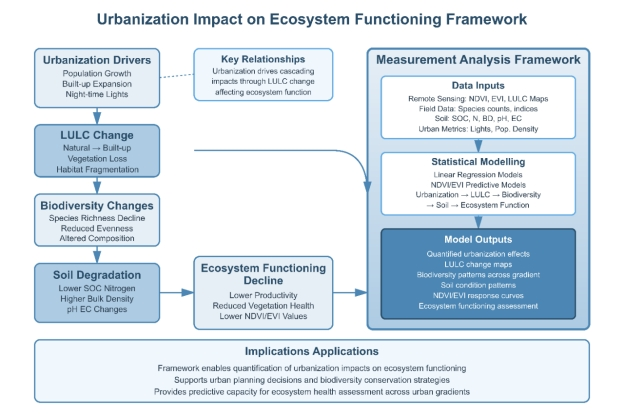
\includegraphics[width=6.5in,height=3.98958in]{figures/media/image1.jpeg}

\textbf{Figure 1.1:} Flowchart of Conceptual Framework: Author source

